
\documentclass[twocolumn]{article}
\usepackage{mathpazo}
\usepackage{microtype}
\usepackage{times}
\usepackage{titlesec} % 1
%\usepackage{sectsty} % "제 1 절" ...

 %%%%%%%%%%%%%%%%%%%%%%%%%%%%%%%%%%%%%%%%%%%%%%%%%%%%%%%%%%%%%%%%%%%%%%%%%%%%%
 %                              My Commands
\newcommand{\bi}{\begin{itemize}}
\newcommand{\ei}{\end{itemize}}
\newcommand{\be}{\begin{enumerate}}
\newcommand{\ee}{\end{enumerate}}
\newcommand{\ii}{\item}
\newtheorem{Def}{Definition}
\newtheorem{Lem}{Lemma}
\usepackage{algorithm}
\usepackage{algorithmicx}
\usepackage{algpseudocode}

\usepackage{graphicx}
\graphicspath{%
        {converted_graphics/}
        {./images/}
}

\usepackage[hangul,nonfrench,finemath]{kotex}
%\usepackage{kotex}    

\setlength\textwidth{7in} 
\setlength\textheight{9.5in} 
\setlength\oddsidemargin{-0.25in} 
\setlength\topmargin{-0.25in} 
\setlength\headheight{0in} 
\setlength\headsep{0in} 
\setlength\columnsep{9pt}
\sloppy 
 
\begin{document}

\title{
\vspace{-0.5in}\rule{\textwidth}{2pt}
\begin{tabular}{ll}\begin{minipage}{4.75in}\vspace{6px}
\noindent\large {\it KIWI Project}@Data Management Research Section\\
\vspace{-12px}\\
\noindent\LARGE ETRI\qquad  \large Technical Report 15ZS1410-TR-43
\end{minipage}&\begin{minipage}{2in}\vspace{6px}\small
218 Gajeong-ro, Yuseong-gu\\
Daejeon, 305-700, South Korea\\
http:/$\!$/www.etri.re.kr/\\
http:/$\!$/sungsoo.github.com/\quad 
\end{minipage}\end{tabular}
\rule{\textwidth}{2pt}\vspace{0.25in}
\LARGE \bf An Overview of MapD \\
\large Massively Parallel Database
}

\date{}

\author{
{\bf Sung-Soo Kim}\\
\it{sungsoo@etri.re.kr}
}

\maketitle

\begin{abstract}
{\small
In recent years, there has been a focus on using distributed clusters of computers to compute aggregates and other statistics for massive datasets. While these approaches, such as the popular MapReduce framework, are invaluable for extracting actionable information from petabyte-sized datasets, such methods typically require large amounts of hardware (even on a per-byte basis) and suffer from relatively high computational overheads due to the large amount of inter-node communication and synchronization involved. Moreover, for medium-to-large size datasets of less than a few hundred gigabytes, such methods introduce latencies that prevent real-time analysis of data, something immensely valuable in diverse fields such as business intelligence, disaster response, and financial market analysis, among others.
}
\end{abstract}

%\begin{figure}[!t]
%        \centering
%        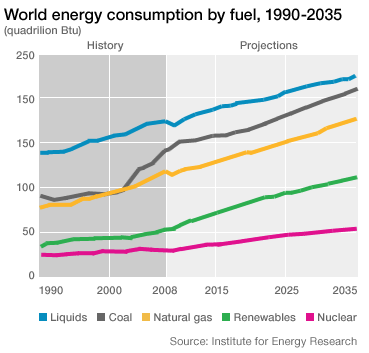
\includegraphics[width=0.33\textwidth]{test}
%        \caption{Caption}
%        \label{fig1}
%\end{figure}

\section{Introduction}
The system described within, \textit{Massively Parallel Database} (MapD), takes advantage of the immense computational power available in commodity-level, of-the-shelf GPUs, originally designed to accelerate the drawing of 3D graphics to a computer screen, to form the backbone of a data processing and visualization engine that marries the data processing and querying features of a traditional RDBMS with advanced analytic and visualization features. As will be shown, MapD is a unique general-purpose modular system that allows for real-time querying, analysis and visualization of “big data” in real-time on hardware ranging from sub-USD1,000 commodity laptops and desktops all the way to High Performance Computing (HPC) clusters with hundreds or thousands of nodes. Moreover, since MapD provides a vertically-integrated end-to-end solution for data querying, visualization and analysis – it avoids latencies that would otherwise be incurred formatting data and needlessly moving it in and out of ultra-fast GPU memory across the relatively slow PCI bus, which would be required if several different (GPU- based) programs were used to perform the same functions, each with their own protocols.

\section{Technical Background}
MapD is a software system that is designed to run on a hybrid architecture of GPUs and CPUs. Every modern computer has at least one CPU, and increasingly computer CPUs are divided into more than one sub-processing unit, called cores. It is not uncommon, as of early 2013, for a high-end laptop or desktop computer to have four cores, and many servers have up to 16 cores. The trend towards more cores has been propelled by the inability of computer chip designers to continue to increase chip clock speeds (i.e. the number of computational cycles a processor can complete per second), as the amount of energy required and heat produced increases super-linearly above a certain point, rendering further increases in clock speeds impractical. To counter this “clock-speed wall”, processor designers have resorted to other means to continue the inexorable exponential increase in processor speeds that both home and business consumers have come to expect. One strategy has been to increase the complexity of chips, improving the chips’ capacity for branch prediction (which allows data to be pre-fetched
from memory before execution) as well as deepening the processor’s pipeline, effectively increasing its throughput.

The other strategy, as hinted at above, has been to increase the number of processing units in a physical chip. Theoretically, twice the number of processors allows for twice the number of instructions to be processed at once and thus provides twice the computational throughput. However, increasing the number of processors introduces a number of complications. First, some algorithms, such as compiling computer code within the same compilation unit, are very difficult to parallelize. Second, even the use of multi-core architectures to accelerate “embarrassingly parallel” architectures typically requires rewriting major parts of an existing codebase to take advantage of the extra cores. In between these two extremes lies the majority of algorithms, those that cannot be trivially parallelized, but with the right (likely non-obvious) algorithm, can still enjoy significant speedups when run in parallel. Such cases typically require even more extensive rewriting of existing code, as the algorithms used to process data may now be completely different than those used in the serial case.

GPUs can be seen as the extreme embodiment of the second approach to overcoming the clock-speed dilemma. The modern GPU evolved in a race to provide the most cost-effective way to perform the massive amounts of computation necessary to render 3D graphics for video and console games – which typically involve hundreds of millions or billions of identical matrix operations per frame to compute the correct projection of vertices in 3D space onto a 2D screen and then fill the resulting polygons using a lighting-dependent shading algorithm.. Hence, emphasis was placed on endowing graphics cards with a large number of architecturally simple cores running at relatively slow clockspeeds, at least relative to the high-frequency, deep- pipelined, heavily-cached world of CPU cores. Moreover, since every core was designed to execute and perform the exact same operation in lockstep with every other core, GPUs ended up being built with a relatively low amount of control architecture, the part of the chip that enables the divergent execution of different branches of code. As such, the first programmable GPU was not offered until 2011, and even modern GPUs do not allow each core to execute independently (Nvidia’s architecture only allows for control at a resolution of 16 threads (processors), called a half-warp).

GPUs compensate for these limitations by using a massive amount of cores. To date, state of the art consumer/gamer GPUs such as the Nvidia Titan might have 2,668 cores and be capable of 5 Teraflops of single precision performance and 1.48 teraflops of double precision performance. Two such cards installed together into a standard desktop computer would be faster than the fastest supercomputer in 2000, the ASCI RED, that took up 1600 square feet of space, used 850 KW of electricity, and cost USD55 million to build. In contrast, the two Titan GPUs described above cost approximately USD1,000 each, use a combined 500 watts of electricity at peak load, and can be easily be housed in a desktop computer system. The disparity between computational speeds over the last decade is due to the disruptive parallel architecture of the GPU. For instance, the performance of modern multicore CPU chips, offered by leading manufacturers such as Intel and AMD, is measured in tens of gigaflops, approximately a factor of 100 times slower compared to modern GPUs at a similar price point.

The scientific community has in particular taken note of the computational potential of GPUs, and currently many workloads such as protein folding and physics simulations are
accelerated using GPUs. However, most of these programs are written as single-use scripts or programs and are not applicable to problems outside of the specific problem domain for which they were designed. Cross-purpose data management software platforms that use CPUs and - GPUs (as well as other massively parallel cards) in tandem to both perform data warehousing and analytic tasks have been slow to develop because:

\bi
\ii The parallelization process for most algorithms is difficult, particularly in the case of a GPU, which has less tolerance for divergent execution than a multi-core CPU;
\ii Contemporary programming languages and paradigms for GPUs are relatively under utilised and do not integrate well with existing codebases. For instance, writing code to run on GPUs requires a working knowledge of un-orthodox coding languages (in the sense that such languages are not typically taught in computer science programs), such as CUDA for Nvidia’s cards or The Kronos Group’s OpenCL;
\ii The database architecture most commonly used in conjunction with discrete GPUs requires the GPU to communicate with a CPU and transmit memory over the Peripheral Component Interface (PCI) bus, which under the current standard (PCI 3.0) can only transfer data at approximately 12 GB per second. Resultantly, by using MapD in conjunction with one or multiple GPUs or CPUs, data can be processed faster than in the case described above where computational speed is limited by the speed that data can be transferred to and from the CPU.
\ii Memory on GPUs is often limited compared to that found on the CPU. For example, state of the art GPU cards may have 6GB of GDDR5 RAM, whereas a high-performance server might have 128GB or even 256GB DDR3 RAM. The relatively limited amount of memory available on current GPUs is currently a serious constraint for GPU programmers.
\ii The majority of contemporary research focuses on the prevailing paradigm employed to process “big data”, Map-Reduce and cluster computing. These take advantage of the scalability and high thoroughput available when using massive amounts of hardware. Alternatively, MapD and a GPU-centric database architecture focuses on the ultra-low latency that can be achieved when processing big data using one or more GPUs.
\ei

As described below, MapD uses many innovative techniques to overcome these limitations.

\section{Description}

MapD uses a hybrid multi-CPU/multi-GPU architecture running across multiple nodes. This architecture allows for the massive parallelization of the querying, analysis, and visualization of big datasets, and results in an increased speed of processing, in the order of multiple orders of magnitude, across many of the various big data workloads common today. The MapD architecture works in conjunction with deep support for GPU-generated visualizations and allows for the practically real-time exploration of many large datasets by
multiple clients in ways that were formerly impossible. MapD utilizes a set of architectural, procedural and programming innovations to contemporary paradigms of big data analysis and computation to achieve ultra-low latency in the processing of big data workloads. Processing times are generally on the order of milliseconds as opposed to seconds, minutes or hours using other contemporary big database paradigms.

The innovative features that are incorporated into MapD are, but not limited to:

\be
\ii MapD is a GPU data analytical system that systematically exploits both multi-GPU architectures and multi-node architectures. Its design mitigates the costs associated with partitioning data both over multiple GPUs and multiple nodes.
\ii MapD uses a three-layer memory hierarchy where GPU memory acts as ultra-fast buffer pool atop of a CPU buffer pool, which in turn sits atop data stored on hard disk.
\ii MapD returns indexes or compressed bitmaps of matching rows from the GPU to the CPU after a filter operation rather than the post-filtered projected rows themselves. MapD thus overcomes the large GPU-to-CPU bandwidth costs associated with transferring these rows over the relatively slow PCI bus.
\ii GPU query functions are fused as much as possible to minimize memory access costs during GPU-assisted evaluation of queries. Previously GPU database designers have resorted to fusing kernels by hand (i.e. combining the ‘>’, ‘AND’, and ‘<’ operators into one function if this is a common workload for the database). In contrast, the first time MapD sees a certain type of query, it actually generates GPU assembly code for a given query plan and then compiles it to allow for the generation of arbitrarily complex fused kernels for queries that could not be anticipated at compile time. After this initial compilation, these compiled kernels are then stored by the system in a dictionary for future re-use so that the up-front cost of query plan compilation is not incurred again. Furthermore, compiled kernels are stored in file, only being deleted if they are not used again within a user-defined number of queries (the user can choose to never delete compiled kernels if disk and memory space is not an issue).
\ii Query optimization for complex queries often involves testing a huge number of possible query plans. Query optimizers found in modern databases typically “give up” after a predetermined amount of time, or constrain the search space to a limited subset of all possible query plans. Both techniques often result in sub-optimal query execution times. To address this issue, MapD experimentally uses the computational power of one or multiple GPUs to determine the optimal query plan for a given query, significantly increasing the number of query plans that can be run-time estimated in a given amount of time, thus increasing the likelihood that the most effective query is found, in turn improving overall system performance. Furthermore, MapD uses its built-in high-performance histogramming capabilities (see 6 below) to improve the statistics that the query optimizer uses (i.e. it improves selectivity optimization)
\ii The creation of an SQL extension along with supporting GPU query architecture to systematically handle the binning (histogramming) of data along an arbitrary number of continuously-valued dimensions, afterwards applying any SQL-standard or user-provided aggregate function, and then allowing for the post-processing of this binned aggregated data
using arbitrary (including user-defined) convolution filters. This allows the database client to request a heatmap of the percentage of data points in a certain area matching a given query in the same way as it allows for the generation of a time graph of minimum, maximum and average temperature for a given map extent. Convolution filters can then be used to perform functions such as spatial aggregation (via gaussian blur or box blur) or finding local extrema in the data. Finally, MapD allows for the systematic export of this post- binned/aggregated/convoluted data into a variety of formats, including but not limited to ordinary tabular format, CSV, JSON (useful when serving as a web server), PNGs (returned for Web Mapping Service requests), and finally as the basis for OpenGL rendering which can either be sent straight to the user’s screen if the MapD server is actually on the same node as the client, or out over a TCP connection via compressed H.264 video (where compression is performed on the GPU).
\ii An algorithm to conduct hyper-fast spatial joins (for example, finding the number of tweets in Texas when the tweets only contain coordinate information). This is done by using the GPU to rasterize in parallel a polygon vector file (such as a shapefile), and then pyramiding it into a lookup tree. Finding the polygon that contains a given point then becomes as simple as looking up the correct pixel in the raster tree and then returning the polygon ID for that pixel. Edge pixels are recorded as such and require an actual intersection test using the underlying vector geometries, but these cases are rare enough so as to have a negligible impact on the overall speed of the algorithm. Preliminary tests have shown speedups of over 1,000,000 times compared to in-memory implementations in PostGIS (a PostgresSQL extension), partly a function of the increased speeds of the GPUs (which are exceptionally fast at texture lookups), but mostly due to the design of the algorithm in question.
\ii A novel algorithm to store the content of text data using the products of prime numbers, leading to both computational speedups and significant data compression. This is called “prime encoding”.
\ii MapD allows for SQL query results computed using its database architecture to be seamlessly passed to various processing modules (such as an included graph analytic package). For example, a user can filter a dataset to filter only those records pertaining to Facebook users from California, and then a compute a real-time 3D force diagram on the results and associated link records, finally passing the data into the provided OpenGL rendering module. One big advantage of MapD’s vertically-integrated architecture as an end-to-end data querying, processing, analytic and visualization engine is that when possible, data never needs to leave GPU memory as it is manipulated by successive (and perhaps fused) kernels. This leads to huge speedups over competing solutions that are more piecemeal, even those that run part of their workloads on GPUs.
\ii A novel algorithm for performing deep geo-location on documents using machine learning algorithms on the GPU. “Deep geolocation” is here defined to be a means at getting a best estimate of the location of a document’s author - where location here is a time-weighted function of their past locations as well as their present position (a user that says “ain’t” might be from the Southern United States - but the fact that they repeatedly say “Eiffel Tower” and “Louvre” may suggest that they are currently in Paris). Previous geo-location systems have only relied on pre-generated dictionaries or gazateers containing place names, ignoring various language features that might provide a clue to the user’s location (for example, the
use of “wicked” near Boston, the use of “bra” instead of “bro” near Atlanta, etc.) The GPU processes a training dataset (such as a dataset of tweets and their geolocations), and then for any document, uses a spatial (2D) Bayesian classifier or other suitable machine learning algorithm to determine probabilities of a user belonging to a given set of N equally sized cell defined by an X and Y extent (a good choice might be a 4X4 grid covering the area in question) The algorithm recursively descends into a given cell if the probability of the document being produced in that cell was higher than a certain amount, stopping when the probability of all sub-bins of a given cell are approximately the same, suggesting that the algorithm could not obtain any more resolution on the document’s location (for example, some users may only be able to be located to the southwest). For other users however, the algorithm may not only be able to determine with high probability that not only are they from New York but also that they frequent a certain bar. The output of the algorithm can be either a probability kernel density heatmap (or pyramid of maps) or explicit probabilities that a user is from a given area represented as a polygon on the map (say a state or census district).
\ii A novel algorithm to determine “trends” in a dataset over any arbitrary extent in time or space. This is currently referred to as “deep trend detection”. Given a weighting function that weights uniqueness in time vs. space, the algorithm essentially uses the computational power available though GPUs to create a 4-D histogram (x, y, time, keyword) of percentage matches for the N most common words in teh dataset as well as the M most common bigrams for a given time and geographic extent. While the top-N unigrams are easy to determine over a given sample, the huge Cartesian space required to represent the space of all possible bigrams (NxN) requires the use of an on-GPU hashing algorithm to keep count of the top bigrams in the limited GPU memory space. It then uses t-tests to test for statistically significant increases in data points for a given term or phrase for a given cell relative to previous time bins for the same cell. The result is then put through a convolution filter to detect geographic blobs - i.e. sets of neighboring cells that all experienced an increase in relative frequency relative to past time bins. If all cells in a given spatial extent experience a similar increase - this is tagged as a trend that is uniform across geographic space. Trends that are confined to a certain group of cells, however, can be plotted on a map. While there are existing technologies to detect geographically-based trends on sources, such as the social network Twitter, due to processing and algorithmic limitations these are limited to only detecting trends in the current time frame and not on-the-fly and in with near-zero latency across time and space.
\ii The integration of a graph analytic module that takes filtered results, upon which various graph statistics can be computed (including but not limited to finding the shortest path length between nodes, the average path length between all nodes, and the centrality of a given node). The module also supports the modeling and rendering of iterative force diagrams of graph data. The results can be rendered in real-time using OpenGL or sent over a network connection as a list of positions or a pre-rendered JPG or PNG.
\ii Fast GPU-accelerated clustering and k-means functionality that can be applied to any result set.
\ee

\section{Technical Details}

There are a number of features used in MapD that have been implemented, to varying degrees, in existing RDBMS and data analytics packages. Occasionally, these have also been implemented as custom programs as part of larger big data paradigms such as the popular Map Reduce Framework. However, MapD, through a number of innovative architectural, procedural and programming features working in unison with existing paradigms of big data and GPU based database computation, creates a novel hybrid multi-CPU/multi-GPU database architecture for the computation of big data.

The base of the MapD system is a hybrid CPU/GPU column-store relational database. A column-store database is a relatively new variant of a traditional RDBMS that stores its data in columns rather than in rows as in a traditional database. This architecture allows for both the more efficient processing of data on the GPU or CPU, or multiple units of both, as well as for optimal use of relatively limited GPU memory. GPU memory is optimized in that the columns, which are frequently used to filter on or aggregate on, can be cached in the memory of the GPU, while the data columns that are not frequently used can be stored in the more-abundant memory located on the CPU.

Contemporary database paradigms are built around the concept of a buffer pool – an area reserved in CPU memory to cache certain blocks of records read from disk. The reason for this is that it is possible to read data from CPU memory orders of magnitude faster than to read it from a hard disk. However, since CPU memory is often smaller by an order of magnitude or more than the space available on a hard disk, it is important to design a database architecture that carefully and effectively selects which blocks of data or records are to be cached in CPU memory. Much research has been conducted on this subject, with various strategies developed to determine which data or records should be cached , or alternatively, which records should be the first to be replaced (via a replacement strategy) when new memory is read from disk to main memory.

MapD is designed with this basic database architecture in mind. However, MapD does not use a dual-level memory model, where data moves between CPU memory and memory on a hard disk. Rather, the MapD architecture implements a three-level model of memory and data synchronisation. This three-level model is arranged in a pyramid, where each successive level of memory is slower computationally but larger in size than the last. The fastest and smallest level is the memory on the GPU, next is the memory on the CPU and, finally, the base of the pyramid, being the slowest but most plentiful, is the memory on the hard disk.

Every level of MapD’s memory hierarchy is a mirrored subset of the level below it. For example, if a given dataset is one terabyte in size, 80 gigabytes of the most frequently used data or records might be mirrored and stored on the CPU memory. Then perhaps the most frequently used 24 gigabytes of those 80 gigabytes will also be mirrored and stored in GPU memory (given perhaps 4 GPUs with 6GB of memory each). See Figure 1 for an overview of MapD’s architecture.


%The atomic unit of memory management in MapD is the “chunk”, a user-definable section of a column, by default set to be 1,048,576 million (2^20) records, equaling roughly 4 megabytes of integers or 8 megabytes of double-precision floating point values. However, the chunk size of variable-length data such as strings (for instance, data strings might hold a sequence of user generated natural language text, among other things) is by default set to be smaller, at 65,536 (2^16) rows. This is because storing variable length data requires both storing the data itself (for example, the component letters in a word, i.e. “h-e-l-l-o”) as well as an indexed offset in the data array to know where a given data entry starts and ends. 65,536 rows is the maximum number that can be indexed with two bytes (a short integer) rather than four (a regular integer), so breaking up variable length data and storing indexed offsets in chunks of this size requires only half as much memory space to store the data’s offsets.
%The size of the chunks involves a compromise. As chunks get smaller, the MapD database is able to distribute data among the three memory levels described above with a greater level of granularity. However, the smaller the chunk, the slower the database can both read the chunk from a hard disk into the CPU memory and the slower it can transfer the
%memory from the CPU memory to the GPU memory and back (since much of the costs of reading and transferring memory can be amortized across the entire length of data being accessed. For example, to begin a new read from a random memory location, disk-based hard disks must physically seek the disk head to the correct position. Since the head is already in the correct position for subsequent reads, these reads can occur much faster).
%In the MapD architecture, each chunk, if taken from a column that allows null values, also has a corresponding bitmap to represent null values. This typically takes only a small amount of space relative to the column itself (1 bit per row so 1/32th the size in the case of 4- byte integers). Further, all chunks for a given set of rows of the same table are combined into a table fragment. In addition to the chunks of its constituent columns, a table fragment also contains a bitmap representing rows that have been deleted from the database (again, requiring 1-bit per row). Periodically, the MapD system repacks a table fragment, removing the rows that are deleted and recompressing each of the table fragment’s constituent chunks. Note that a table in itself can be composed of any number of constituent chunks. See Figure 2.
%Figure 2: The structure of a sample database table, split into M fragments, each which is split into N chunks, each with its own bitmap to record null values (if the column permits nulls). Finally, each fragment keeps a bitmap to record row deletions. The columns of fragments are periodically compressed by removing rows that are flagged in the row deletion bitmap.
%There are two ways in which MapD can partition data. The first, the round-robin method, essentially takes an incoming row of data (inserted either via SQL “insert” syntax or by binary batch insert), splits the row into its constituent columns/fields, and writes each to the appropriate chunk of a table fragment for that column inside the CPU memory. These chunks cannot be moved to the GPU until full, until then – they are queried on the CPU. This prevents the costly memory overhead of transferring every record to the GPU and allows for the batching of transfers for greater net throughput. Note, however that updates and deletions to chunks on the GPU must be recorded on the GPU immediately – as queries on these “mature” chunks run on the GPU and thus could return inaccurate results if the null and deletion columns are not kept up-to-date on the Gpu memory. After this initial “incubation” stage in CPU memory, all chunks for a given column are treated as equals, with the database only keeping statistics on which columns are accessed more, keeping the chunks of these columns higher in the memory hierarchy. However, the user can issue a command to declare that the chunks of a given column should always be, or alternatively, never be held in GPU memory. This can be useful in cases in which the user requires queries for certain columns to run at a given speed, or when due to the data requirements of a certain application (such as prior knowledge that the latitude and longitude columns of a table will be always used when rendering heatmaps of datasets that include geo-location data), the user knows that certain columns will be involved in every query and does not want these columns to ever be moved off the GPU memory.
%The second method is via explicit clustering of the data by the values of one or more variables (columns) of a table. MapD allows the user to choose the number of partitions as a settable parameter, but in default mode MapD dynamically chooses the number of partitions for a given table given both the table size and the query workload. All things being equal, the more rows a table has the more partitions it can viably support. Partitioning can be setup to run in simple mode, in which the data of the column to be partitioned on is sorted and then split into N sections. The average value of the maximum value of one partition and the minimum of the next is then chosen to be the partitioning point. So if table T is partitioned along column A, which as 100 values [1..100], and the number of partitions is chosen to be 4, partition points will be chosen at 25.5, 50.5, and 75.5. Alternatively, table partitioning can be done taking into account past query history, with the goal of clustering data that tends to be accessed together (by the same query) so as to minimize memory accesses and the number of GPU kernel functions that must be run.
%Clustered partitioning based on query history allows for the following:
%1) Since we know the range of values each clustered column in a table fragment can take, we do not need to scan table fragments with clustered column values outside of this range. This can lead to major speedups
%2) Table fragments corresponding to different clustered column ranges can be placed on different GPUs, maximizing the probability that one GPU in a multi-GPU system can handle a query by itself (the other GPUs in the system can be handling their own queries) - removing the cost of merging each GPUs result set (whether an aggregate value, a heatmap, or a table of data sorted on some value).
%HOW MAPD PROCESSES QUERIES
%Although the architectures for several GPU-accelerated databases have been laid out in various academic papers, these systems typically work on the assumption that the data to be queried always resides on the GPU, which may be an unrealistic assumption for real-world query workloads and database applications, or that data is just blindly streamed to and from main CPU memory query, leading to only modest speedups due to the disproportionate time that CPU-to-GPU and GPU-to-CPU transfers over the PCI bus require relative to GPU execution time. MapD allows for the streaming of data to-and-from the systems GPUs such that there is no “cap” on the maximum amount of data that can be processed for a given query. However, unlike previous systems, it attempts to minimize PCI transfer by only sending compressed bitmaps or index maps of post-filtered results across the bus. Furthermore, since GPU and CPU execution can occur asynchronously, MapD’s query planner runs query workloads that run relatively faster on the CPU, such as text query using an inverted index, on the CPU while performing queries that run relatively better on the GPU, such as brute force table scans, simultaneously on the system’s GPU(s).
%The following steps through what occurs when a typical SQL query arrives to the system, whether over a normal TCP connection or as part of a HTTP request via MapD’s REST or Web Mapping Service (WMS) APIs (see Figure 3 at the end of this section for more detail).
%1) The query is parsed and an Abstract Syntax Tree (AST) is produced according to established practice, with one node per abstract operation on the data;
%2) The query optimizer attempts to determine the quickest way to execute the query, taking other query load on the system into account. To do this, it must determine which chunks are in GPU memory, CPU memory, and on a hard disk. As noted above, it attempts to separate the query plan into parts and process on the GPU and CPU those parts that are most relatively faster on those components. It also must determine which parts of the query are dependent on intermediate result sets being materialized and generate plans accordingly.
%a) Query optimization requires accurate statistics on the distribution of data within a given table to produce good results (i.e. to estimate how many result tuples will be produced by a given filter operation). To that end, MapD works to keep up-to-date statistics (histograms) of the data it stores (selectivity estimation) - using periods of low query activity to analyze ist data using the same query architecture it uses to handle actual queries produced by clients (i.e. it runs query simulations).
%b) During this optimization process, the query optimizer can reorder the AST to the extent allowed by the rules of relational commutativity to speed up the query. This often involves “pushing” operations like filters to the bottom of the tree so that any joins (typically costly) occur over the minimum amount of records possible.
%c) Given a complex enough query, the number of possible query plans can become extremely large, increasing exponentially with every new node in the AST. Given such queries, modern databases will typically estimate execution times for only a fraction of the total possible query plans, attempting to find a “decent” query plan if not a globally optimal plan. To address this shortcoming of traditional database architectures, MapD uses the system’s GPU(s) to speed up query plan evaluation, greatly increasing the number of possible query plans that can be considered by a database over a certain amount of time.
%3) Using a hash of the chosen query plan (including the data types of the columns to be queried/processed), the database then checks to see if it has stored compiled GPU and CPU code to execute the query, which it stores in a dictionary mapping function definition hashed to function pointers to compiled code. If it has the compiled code cached, it immediately executes the query plan. If not, MapD will then generate GPU and CPU assembly code based on the general query plan. (Sometimes only one part of a query plan will need to be compiled) To the extent possible, it attempts to create a single fused function/kernel for the entire query plan. Sometimes this is not possible and intermediate data must be materialized (i.e. written to memory - a relatively resource costly process), before starting a new kernel to continue processing the query (this frequently occurs in the case of joins, where post-filtered results from both join tables must be written to memory before evaluating the join. Once the assembly for the kernel is generated, it is linked using existing compiler functionality (for example, nvcc for Nvidia’s CUDA API) and a function pointer to the kernel is stored in the kernel dictionary described above. Thus, compiling code for a novel query entered into the system is only an up-front cost, which due to the pre- compilation of assembly code performed by the database itself is a relatively fast process.
%4) The compiled kernels are then executed - typically simultaneously on the node’s CPUs and GPUs, according to the query plan.
%5) The last part of the query plan may involve computing aggregates on the filtered and joined data. If so, then this generally results in a result set that only occupies a tiny fraction of memory that the original dataset and the resource overhead of GPU-to-CPU memory transfer is negligible. However, there are cases in which the user requests one or more non- aggregated columns. Within other constraints, MapD endeavours to minimize GPU-to-CPU memory transfer due to its relatively resource costly nature. GPU-to-CPU memory transfer generally falls into the following subcategories:
%a) After the computation of aggregates, as described above, these aggregates (whether the product of a GROUP BY or a BIN BY query (described below) - normally have a small memory footprint relative to the dataset they are derived from. In such cases the resource overhead of PCI memory transfer is negligible.
%b) The query involves filtering by some criteria but the projected columns are returned unaltered (for example, the query “SELECT * from geo_tweets where lat > 30.0 and lat < 50.0 and lon > 30.0 and lon < 50.0 and time > ‘2012-08-01 11:54’ and time < ‘2012-08- 02 11:54’, the * telling the database to return all columns that match the filter criteria unaltered). In such cases, the database only needs to return the indices of the rows of the table fragment that pass the filter test rather than all of the projected columns. If the percentage of results relative to the entire result set is high, it may make most sense to return a bitmap of the matching rows, one bit per row, where each bit is set to either True or False depending on whether the row passed the filter test. The bitmap has the advantage of being the raw form that the GPU uses to compute results, with each thread in the GPU writing its row’s result directly to that row’s indexed offset in the bitmap, requiring no thread coordination. However, if the result set is a small percentage of the total dataset, it may make sense to only return the indices of the matching row in integer form, which is generated from the bitmap described above via a parallel prefix scan. Furthermore, the database can run-length encode (compress) these indices (currently implemented with Rice Encoding) to save even more bandwidth. For instance, in a case where a filter operation on a billion rows only returns one thousand results. Instead of returning a billion-bit bitmap (1 billion/8 ~= 125 megabytes), the database would only have to return 1,000 4-byte integers (4 kilobytes). Aside from the drastically lower bandwidth required to transfer the indexed list from GPU to CPU, the CPU also now has a much smaller result list to scan. However, to transform the raw bitmap into a list of integer indices, a relatively costly parallel-prefix scan operation must be performed. The actual strategy chosen taken at query time is left to the query optimizer, which makes its decision based on estimated costs of each step (in turn based on computed statistics of data distribution as well as other benchmarks (such as the actual PCI transfer speed of the system in question as well as the relative difference between GPU and CPU processing power).
%c) The query involves the computation of derived results on the post-filtered projected columns. This means that all derived columns computed on the GPU, and not just the indices of the rows that pass the filter test, need to be returned to CPU memory. If a LIMIT clause is invoked (limiting the number of rows returned), only the specified number of derived rows need to be returned, lessening the bandwidth transfer. MapD’s
%Figure 3
%query optimizer will push more computational load on the CPU to compensate for the increase bandwidth required as needed.
%
%BINNING/HISTOGRAMMING + CONVOLUTION FUNCTIONALITY
%While the current SQL standard allows for aggregation by discrete values (via the GROUP BY) operator, it is very difficult to easily specify the creation of arbitrary histograms across an arbitrary number of dimensions, each a continuous variable. Consider the following use case: the client wishes to generate a heatmap showing the average temperature over a given geographic extent for a certain time range. Although this is possible using ordinary SQL, generating such a query is incredibly unwieldy. The SQL query to perform compute the data necessary to populate such a heatmap is the following:
%
%Expr 1
%SELECT (x - $x_min)/($x_max - $x_min) * $num_x_bins AS x_bin, (y - $y_min)/($y_max - $y_min) * $num_y_bins AS y_bin, COUNT(*) AS N, AVG(temp) AS avg_temp FROM weather WHERE date >= ‘2012-07-01’ AND date <= ‘2012-07-07’ GROUP BY x_bin, y_bin HAVING $x_bin >= 0 AND x_bin < $num_x_bins AND y_bin >= 0 AND y_bin < $num_y_bins AND N > $min_n;
%This query bins the data into a 2D histogram (by x and y) for all weather observations for a given spatial and time extent. The number of bins, as well as their bounding points, is determined by the variables $x_min, $x_max, $num_x_bins, $y_min, $y_max, and $num_y_bins. Note that the HAVING clause, aside from limiting the result set to the correct bins, also performs a post aggregation filter on each bins count (aliased to N), specifying that the cell has at least a minimum number of observations ($min_n) for the bin to be included in the result set.
%Now consider MapD’s histogram functionality. In MapD, the query above could be expressed as:
%Expr 2
%SELECT x, y, COUNT(*) as N, AVG(temp) as avg_temp FROM weather WHERE date >= ‘2012-07-01’ AND date <= ‘2012-07-07’ BIN BY (x, $x_min, $x_max, $num_x_bins), (y, $y_min, $y_max, $num_y_bins) HAVING N > $min_n;
%Note how the BIN BY operator, given the appropriate minimum, maximum, and bin cardinality parameters for each dimension, automatically allows for the computation of the appropriate bin of the data (performed as a projection in the SQL query), in addition to handling the bounds checking performed by the HANDLING operator in the SQL query.
%While the example above computes a binned aggregate across two dimensions (the variables x and y), the same methods abstract to any number of dimensions. For example, the user can generate a time graph of the percentage of tweets matching a given query term via:
%Expr 3
%
%SELECT time, AVG(tweet_text ilike ‘%$query%’) from tweets BIN BY (time, $time_min, $time_max, $num_time_bins);
%Or alternatively, a 3D histogram of batting average for batters against a certain pitcher, binned by the x and y coordinates that the ball crosses the plate and the speed of the pitch:
%Expr 4
%SELECT x, y, speed, AVG(was_hit) FROM at_bat_stats WHERE pitcher = ‘$pitcher_name’ BIN BY (x, $min_x, $max_x, $num_x_bins), (y, $min_y, $max_y, $max_y_bins), (speed, $min_speed, $max_speed, $num_speed_bins);
%Note that when using this functionality to render two-dimensional heatmaps for on- screen-display, the number of bins in each dimension often equals the size in pixels of the frame being requested from the MapD server.
%MapD also allows for the integrated specification of convolution filters that are run on the post-binned data. A convolution filter applies a given function on every bin in a histogram over any number of dimensions. Typically the input into the convolution filter for a given bin is the bin’s value along with the values of any number of neighboring bins. The convolution filter can optionally be parameterized such that it only considers the N closest bins along any given dimension.
%MapD allows for the user-defined convolution filters. Typically this is done by providing MapD with a D-dimensional matrix that expresses the weights that each bin within a [N0,N1... ND] bin neighborhood of a bin contributes to the new value for that bin. However, the user can also provide a coded User Defined Function (UDF) to perform custom operations not expressible by a convolution matrix.
%Convolution functions in MapD are defined using the CONVOLUTE operator, which is applied to the result of any bin operation using nested query syntax. Taking our previous example of the computation of average temperature across a geographical region:
%Expr 5
%SELECT CONVOLUTE(SELECT x, y, COUNT(*) as N, AVG(temp) as avg_temp FROM weather WHERE date >= ‘2012-07-01’ AND date <= ‘2012-07-07’ BIN BY (x, $x_min, $x_max, $num_x_bins), (y, $y_min, $y_max, $num_y_bins) HAVING N > $min_n, GAUSSIAN($sigma), 100, 100);
%The first thing to note is that the inner query of this example is the same as the query in Expr 2. However, this inner query is wrapped in a convolution query. The first parameter specifies the input(required to be an SQL function with the BIN BY operator), the second parameter is the convolution function to be applied (a Gaussian blur in this case) – optionally parametitized, here $sigma is the standard deviation of the blur function (the second parameter
%can also be a matrix rather than a named function as described before). Finally, the parameters 100, 100 specify the maximum convolution window (in x and y) that should be considered in determining any bin’s post-convolution output value.
%The output format for a binning/histogram query can be specified by the user/client. This is useful because frequently, the goal of a binning query is to generate a visualization, whether rendered as a static image and returned to a web browser, or perhaps pushed into the GPU’s graphics pipline for real-time manipulation in 3D, or alternatively, rendered as a video (for example, animating using the third time dimension of a heatmap over some spatial extent defined over the variables x and y). By default, the results of the binning operation are pushed back to the CPU (for queries that run on the GPU). However, the exact output destination (as well as relevant parameters) can be specified via the OUTPUT TO operator that is placed at the end of the full query. Current options include but are not limited to OUTPUT TO TABLE (default), OUTPUT TO CSV, OUTPUT TO JSON (useful for web clients), OUTPUT TO PNG, OUTPUT TO JPEG, OUTPUT TO MP4, OUTPUT TO H264, OUTPUT TO OPENGL and OUTPUT TO DIRECTX. (The program allows for its users to write modules to output to any other format as well). For the image formats (PNG and JPEG), the data must have been binned over either three or less dimensions. For the image and video output options, the system by default (or explicitly set using PROJECT TO HEAT) depicts the “dependent” variable on a color gradient, specifiable either by naming a colorramp preset or by providing a list of 4-member tuples [% maximum, [red, green, blue]] where % maximum lies within the range [0-100], while [red, blue, green] are each specified between [0-255]. However, when provided the PROJECT TO RELIEF parameter, the system instead renders the output with the dependent variable projected into another dimension. Thus a graph of some aggregated attribute against time becomes a proper time graph, while an aggregate binned over two dimensions becomes a 3D relief map. With relief maps, two independent variables can be depicted simultaneously by using “height” to show the distribution of one and “color” for the other. In general, only histograms over two dimensions or less can be rendered as relief maps, and 3D maps over two independent dimensions requires the use of OpenGL or DirectX on the GPU for 3D rendering.
%In addition to linear, log, standard deviation, and other scalings supported by all output formats (specified by including the appropriate function in the SQL (or other supported query format) itself – i.e. LOG(AVG(Z) or STD_DEV(AVG(Z)), the heatmap output option supports Jenks clustering as well as other scalings that require a binned (i.e. non continuous) output/dependent variable. Also, in the case of the PROJECT to HEAT option, the system allows for the client to request a legend identifying how each color or range of colors matches with each range of values in the output data. This can be outputted either in raw data format (i.e. JSON), or as an actual png image for the client.
%OUTPUT TO OPENGL and OUTPUT TO DIRECTX allow for the output of the histogram to a 3D Graphics context, after which the context can be manipulated in real-time using mouse or other input methods (such as a joystick). This is possible since context switching between GPGPU compute APIs such as CUDA and OpenCL and GPU rendering APIs such as OpenGL and DirectX is very quick. This is particularly useful when attempting to view a three- dimensional histogram. In such a case, the computed histogram can be made semi-transparent
%(the degree of transparency controllable by the user in real-time) and then manipulated (rotated and translated), as well as cut into cross-sections, in real time. Note that this mode requires a monitor to be connected to the GPU server so that the OpenGL or DirectX API can output directly to screen. Also note that OUTPUT TO PNG, OUTPUT TO JPEG, OUTPUT TO MP4, and OUTPUT TO H264 may also use either the OpenGL or DirectX APIs for rendering, except that instead of rendering the output directly to screen the rendered buffer in GPU memory is transformed into the appropriate output format and then sent out over a network connection.
%Until now only the system’s capabilities to generate and output binned histograms, as well as the interface it provides for clients to access such capabilities, have been described. While this interface allows for the generic specification of a histogram to be generated over an arbitrary number of dimensions (i.e. an arbitrary set of continuous variables), there is a fair bit of specialization in the back-end application (MapD) to handle such requests in the most efficient manner possible to maximize throughput and minimize latency.
%Much of this specialization revolves around attempting to take advantage of higher- speed shared memory on the GPUs, which is much faster than a GPU’s global memory but also typically much more limited in capacity. Shared memory is specific to each Streaming Multiprocessor (SM in Nvidia and ATI terminology), To do this, MapD first must programmatically determine the amount of shared memory and global memory on all GPUs installed on the host system. Then, when a client request to generate a binned histogram arrives to the system, MapD determines if there is enough shared memory capacity to generate the histogram in shared memory rather than global memory. If there is enough shared memory to construct the histogram of the user-requested size, MapD uses shared memory, merging each SM to global memory as a final step. Otherwise, each GPU thread writes to global memory.
%Figure 4, Figure 5, and Figure 6 depict real examples of MapD-generated heatmaps, point maps, and time graphs for queries over hundreds of millions of tweets. Note that pointmaps are also generated using the binning and then convolution filter method outlined above (in this case, marking the bin as inside a “point” if any any bin within a user-defined raidius has a matching tweet count greater than zero. All of these maps were generated within milliseconds on a 4-GPU system, orders of magnitude than a CPU-only system could accomplish the same task.
%Figure 4- Pointmap, Heatmap, and Time Graph showing flu outbreak in December 2012 in the American South
%
%Figure 5 – Heatmap and Pointmap of tweets containing “Central Park” near Manhattan. The heatmap shows the percentage of tweets containing the place name, suggesting the utility of the “deep geolocation” method described above.
%Figure 6 – Heatmap and time graph of percentage of tweets containing the word “snow” in December 2012
%Figure 7 – Heatmap of points per shot over x and y court position for nearly one million NBA shots.
%SYSTEM OF USING RASTERS TO TEST FOR SPATIAL INTERSECTIONS
%At the core of MapD is a system to rasterize vectorized polygon input such that spatial lookups can be performed near-instantaneously. This system currently takes ESRI shapefiles, an industry-standard format to represent geospatial data (polygons, lines and points) and maps each of the polygons contained in the file to a texture file of user-specified dimensions, with each “pixel” containing an integer value specifying the ID of the polygon at that pixel. This ID can then be joined with a table packaged with the shapefile in dbf format to get the name and other attributes of the polygon. To determine the “parent” polygon of a point, the point is simply projected onto the map and the ID value for that pixel fetched. A further refinement of the system involves pyramiding the raster into a raster tree - where each pixel references a 16X16 child raster. If a pixel lies entirely inside of a polygon, the ID of the polygon is simply recorded at that branch of the “tree” terminates. Otherwise, an offset to the start of the pixel’s child raster is recorded. Such a method saves a significant amount of space at the extent of requiring the GPU to perform multiple texture lookups per query. Since real-world polygons are not neatly defined by square pixels, the tree is terminated at a certain depth for a given pixel if the pixel at
%that point is not entirely inside a polygon (which might occur if the centroid of a pixel lies exactly on a polygon edge). If 100% accuracy is not required, the database can report these points as lying on a polygon edge and not determine the actual container polygon for these “edge” cases (with a sufficient sized raster tree, this typically only occurs for < 1% of points). However, if 100% accuracy is required, the system can then perform a standard spatial intersection test on the edge cases, restricting the candidate polygons to those that border the edge in question. Although the method of testing for point-to-polygon intersections is described here, lines or polygons can also be tested for intersection in the same matter by looking up their constituent points. As noted above, speedups of over 1,000,000 times result from using this algorithm on the GPU versus an in-memory implementation of spatial joins in the popular PostgreSQL GIS extension PostGIS.
%It is notable that MapD can rasterize polygons in parallel. This is done using the following algorithm:
%(a) Preparing table containing the coordinates of a polygon’s vertices and the id of the owner polygon for those vertices
%(b) Using one GPU thread per pair of vertices, determine and store the number of pixels that like between the two vertices given the desired raster size
%(c) Use a parallel prefix scan to compute each thread’s correct memory offset to write the edge pixels that lie between the pair of vertices to
%(d) Each GPU thread now determines the actual edge pixels that lie between its pair of vertices and writes them into its assigned memory slots given by the offsets determined in c)
%(e) Sort this output by polygon id and then by row
%(f) Assign each thread to an outputted edge pixel – the thread then writes to
%memory True if the previous pixel is on a different row, signifying the start of a
%new row.
%(g) Again use a parallel prefix scan to build a dense index of the offsets into the
%edge list of the start of every row by polygon.
%(h) Assign a thread to each of these offsets, which will scan until the next offset
%(representing the next row for the polygon)
%(i) During the scan, the thread will increment an “edge” counter every time it
%encounters an edge on that row.
%(j) If the edge count is odd, the thread fills in the X by Y raster (representing the
%rasterized map) with the polygons id until it encounters the next edge
%Figure 8 - a (visualized) example of MapD’s rasterization of a shapefile containing world polygons
%PRIME ENCODING
%At its most basic level, text search/Information Retrieval (IR) usually involves converting text to an inverted index in which each word is a key for a sorted list of all document ID’s containing that word, perhaps with the addition of information about where the word was found in the document. Although inverted-lists can be compressed to less than one byte per document ID per index term using some algorithms, there is a significant computational cost to decompressing such data which varies by the compression method used. Moreover, due to the serial nature of such run-length compressed listings, it is difficult to efficiently access inverted lists on the GPU unless done as batch queries.
%MapD instead uses products of primes to encode text. To do this, a sample corpus is first generated that is seen to represent the type of text to be encoded. The unique set of words from the corpus are then ordered according to their frequency of occurrence in the corpus. Each unique word key is then assigned a prime number such that the most frequent word is assigned the prime number “2”, the next most frequent (usually “the”), “3”, and so on. The word frequencies can be recomputed at any time and new prime encodings generated for each document to reflect the new ordering, although this is found to be of limited effectiveness after a fairly small corpus is ingested due to the relatively static nature of the relative frequencies of unigram use in language. This set of associations between word key and prime number value is then kept in memory as a hash map. Then, to encode a document, MapD looks up the prime value for each word in the document text, multiplying that value by the product of the primes of all words that came before it. These products are stored as sets of unsigned 8-byte integers; when none of the integers in a document’s existing set can be multiplied by the next prime without overflowing a new integer is added to the set. Then, when MapD needs to test whether a certain word is in a document, it simply looks up the word’s prime in the hash map and then divides each prime product (the 8-byte integers) by the word’s prime, testing for a zero
%remainder (signifying that the word was in the document). In practice, a bit-shift trick is employed that is significantly faster to compute than the relatively costly modulo operation.
%In practice, prime-encoding text results in significant compression of the text, reducing the approximately 80 bytes of UTF-8 encoded text to an average of 15.07 bytes or less than two unsigned long integers, besting the bytes per word ratio of the best inverted index compression techniques by a factor of three. This is the case even though only one prime hash map was used for all languages in the Twitter dataset, which contains significant non-English content. Further compression could be likely achieved by using different hash maps for different country groups (easily achieved using MapD raster lookup system) such that a prime mapping for the Arabic countries would associate common Arabic words with low primes, thus achieving greater compression. Also, common IR techniques, such as removing common words such as “and” (stopwords) and stemming tokens (i.e. transforming cars à car) would significantly reduce the total memory footprint required. Finally, an algorithm is constructed that would dynamically rearrange prime products to minimize the number of 8-byte integers needed to encode a given document. See Figure 10 for a depiction of how prime encoding works to encode and query a sample document “To you, I’m Me.”
%Figure 9 – Prime Encoding

\bibliographystyle{IEEEtran}
\bibliography{References}























































\end{document}
